
In \cref{sec:ramsey} we computed the value of $T_2$ but we overlooked something: from Chapter 5 of Nii Quantum Information Lectures~\cite{nii_quantum_lectures} we read:
\begin{paragraph}
"\textit{An applied DC field $H_0$ is not completely uniform in all space points. If many spin qubits are placed in such an inhomogeneous DC field, they have different Larmor frequencies. This leads to the dephasing effect if we compare the phase difference between different qubits. A time constant for this dephasing process is determined by the spatial (not temporal) inhomogeneous broadening of the dc field and distinguished from $T_2$ process. A new time constant is often referred to as $T_2^\star$.} "
\end{paragraph}

This sentence is not immediately clear, but it is basically saying that a spurious DC field, coming from the other qubits near the one under analysis, or from a near flux line or again just from noise, can lead to an additional dephasing effect not included in the standard definition of $T_2$.
In \cref{sec:ramsey} we did not consider any of these effects, so we actually measured $T_2^\star$ that is a good approximation of $T_2$ in a nearly-noiseless environment.

To measure the pure dephasing $T_2$, we have to perform higher order experiments that take into account these potential impurities. 
One of these is the \textit{Hahn’s spin echo} experiment~\cite{Hahn1950}.\\
The experiment can be seen as a non-detuned Ramsey experiment with the addition of a \pipulse between the two \pihpulse, in particular the experiment is as follows:
\begin{itemize}
    \item a \pihpulse is sent to the qubit so that the state of it is now $\frac{\ket 0 + i\ket 1}{\sqrt{2}}$;
    \item we wait for $\Delta t / 2$ so that the state is $\frac{\ket 0 + e^{-i\Delta t /2}i\ket 1}{\sqrt{2}}$;
    \item a \pipulse is sent to the qubit. The state is now $\frac{\ket 1 + e^{-i\Delta t /2}i\ket 0}{\sqrt{2}}$;
    \item we wait for $\Delta t / 2$ so that the state is $e^{-i\Delta t /2}\frac{i\ket 0 + \ket 1}{\sqrt{2}}$;
    \item we apply a \pihpulse so the qubit reaches $e^{-i\Delta t /2} \ket 0$;
    \item finally, we measure the qubit state.
\end{itemize}

The main difference with Ramsey, the \pipulse in the middle of the experiment, guarantees that any DC impurity applies the same phase to $\ket 0$ and $\ket 1$, therefore leading to a negligible global phase.

We can now perform an exponential fit where we can extract the decay time $T_2$.

Note that there are some experiments of even higher order that take into account other possible impurities, but in general Hahn's spin echo is the used technique for $T_2$.
These experiments include the \textit{Carr-Purcell sequence} and the \textit{Meiboom-Gill sequence}~\cite{PurcellGill}.

Also note that, in literature, there is the tendency to write both Ramsey-$T_2$ and Echo-$T_2$ simply as $T_2$ so one has to be particularly careful when talking about the dephasing time.

A plot for a Echo experiment is presented in \cref{fig:echo} and is, as the ideal Ramsey, a simple exponential decay. However, this time the starting state is $\ket 0$, so the curve is flipped horizontally.

\begin{figure}[ht]
    \makebox[\textwidth][c]{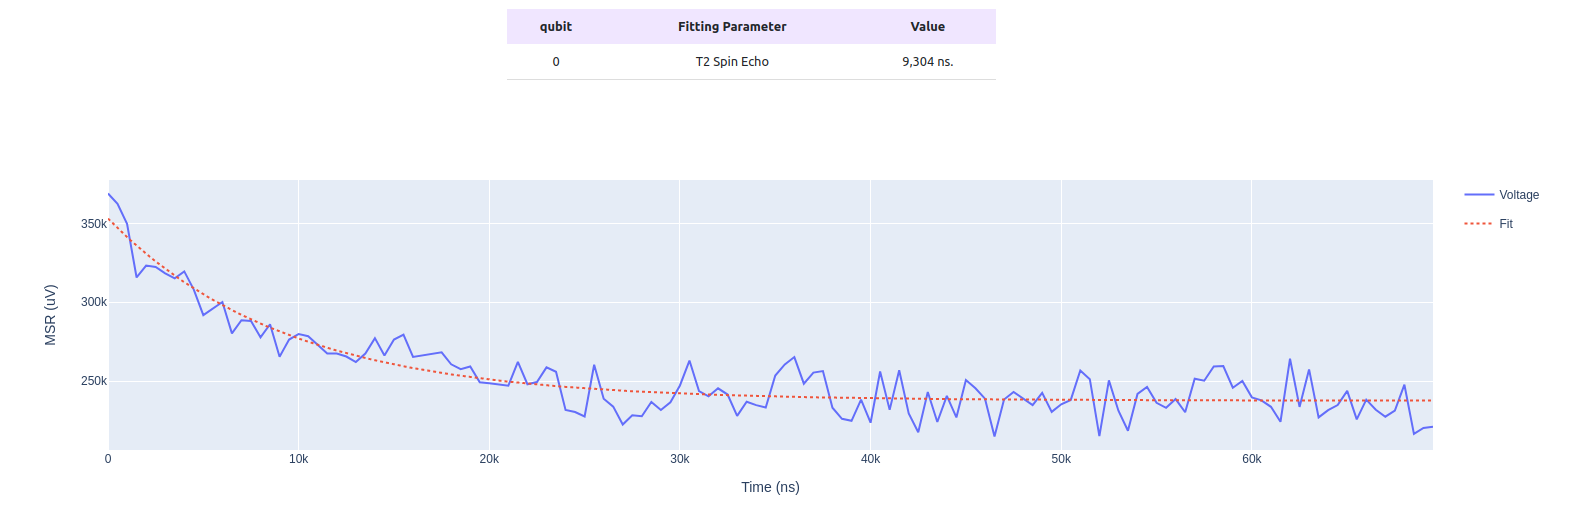
\includegraphics[width=1.3\textwidth]{characterization/figures/echo.png}}
    \caption{Plot of a Hahn's Spin Echo experiment.}
    \label{fig:echo}
\end{figure}


\experimentrecap
{Hahn's Spin Echo experiment}
{qubit characterization}
{characteristic dephasing time $T_2$}
{a \pihpulse is sent to the qubit through the drive line, after a variable wait time $t/2$ we execute a \pipulse and wait again $t/2$. After a new \pihpulse we measure the qubit state.
We can now fit the obtained curve with an exponential curve and obtain $T_2$ as the decay constant. This experiment differs from Ramsey for the introduction of a \pipulse between the two \pihpulse that enables the removal of a spurious dephasing term linked to external DC currents, leading to better estimations of $T_2$}